% arara: lualatex: { interaction: nonstopmode, synctex: no }
% arara: lualatex: { interaction: nonstopmode, synctex: no }
\documentclass[a4paper,12pt,chapterprefix=false,bibliography=totoc,listof=totoc,book]{scrreprt}

\usepackage{latex-style}

\lstdefinelanguage{Gherkin}{
    morekeywords = {
        Given,
        When,
        Then,
        And,
        Scenario,
        Feature,
        But,
        Background,
        Scenario Outline,
        Examples
    },
    sensitive=true,
    morecomment=[l]{\#},
    morestring=[b]",
    morestring=[b]',
    keywordstyle=\normalsize\bfseries\color{green},
    basicstyle=\small\ttfamily,
}

\setlength{\parindent}{0pt}
\newabbreviation{na}{N/A}{Not applicable}

\begin{document}
    \begin{flushright}
        GameBase
        \\
        Use-Case Specification: Show Game Server List (Dashboard)
% \\
% For <Subsystem or Feature>
        \bigbreak
        Version 1.1
    \end{flushright}

    \tableofcontents

    \chapter{Use-Case: Show Game Server List (Dashboard)}

    \section{Brief Description}
    The use case describes
    \begin{itemize}
        \item how a user can inspect their list of game servers
        \item how a user can display details about a game server/container
        \item the controls available for each game container
        \item what happens if a user deletes a container
    \end{itemize}

    \chapter{Flow of Events}
    \begin{figure}[H]
        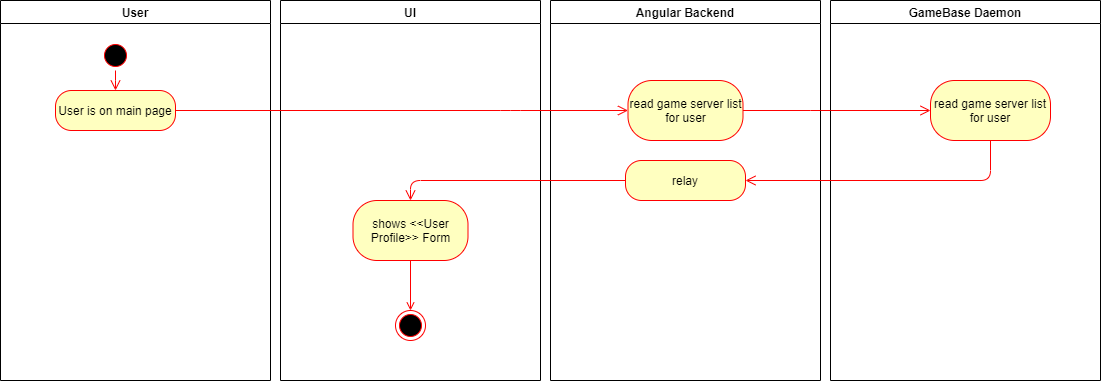
\includegraphics[width=\textwidth]{diagramms/UCShowGameServerListDiagramm.png}
        \caption{Activity Diagramm}
        \label{fig:ucd}
    \end{figure}
    \section{Basic flow}

    \begin{itemize}
        \item User is shown a list of their game servers
        \item They can click on one of the game server (displayed as accordion items) to display more details
        \item Each item in the lists consists of a header and a body.
        \item The user is able to <<Start>>, <<Stop>>, <<Restart>> and open <<Configuration>> of the respective game container.
        \item Next to the server controls, the current status of the respective container is shown.
        \item Further details inside of an item's body include description, assigned resources and a <<Delete>> button. These are shown in the body of an item.
        \item If a user decides to delete a game container, its item will be removed from the list.
    \end{itemize}

    \section{.feature File}
    \begin{minipage}{\textwidth}
    \lstinputlisting[language=Gherkin]{features/showGameServerList.feature}
    \end{minipage}

    \section{Imagery}
    \begin{figure}
        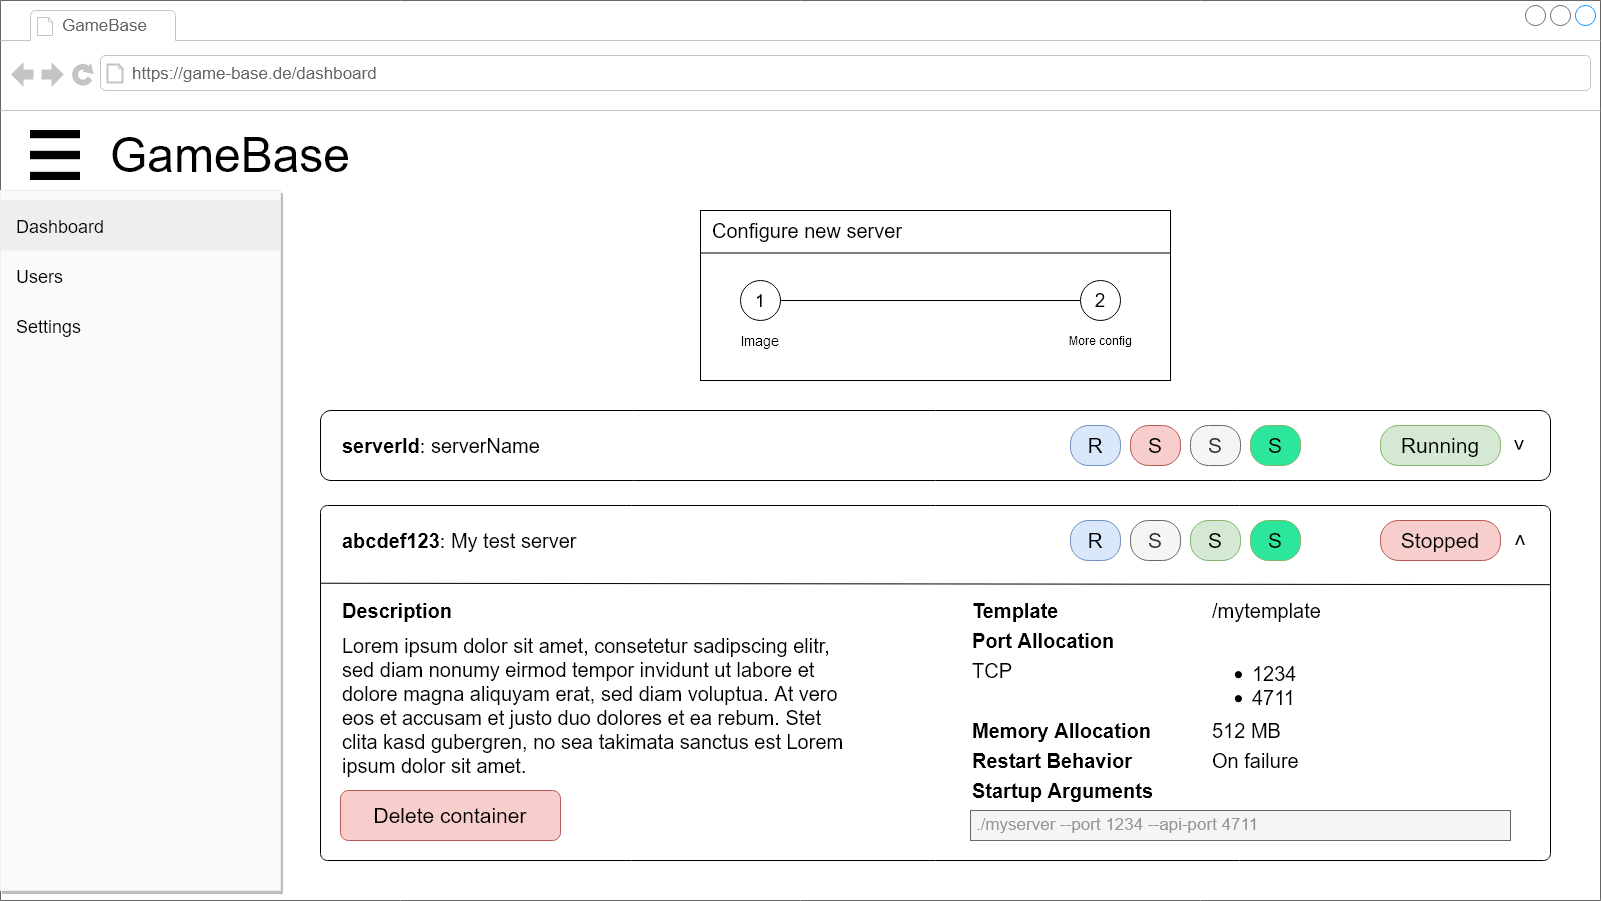
\includegraphics[width=\textwidth]{diagramms/UCShowGameServerListMockup.png}
        \caption{Mockup of the game server list. It consists of the game server creation wizard and an accordion.}
        \label{fig:mockup}
    \end{figure}

    \chapter{Special Requirements}
    \section{Owning an account}
    The user has to be a registered user for our system.

    \chapter{Preconditions}
    \section{Must be logged in}
    The user has to be logged in order to have their servers displayed on the Dashboard page.
    \section{Must be on the Dashboard page}
    The list is available on the Dashboard page.
    
    \chapter{Postconditions}
    \gls{na}
\end{document}
